\documentclass[10pt,a4paper]{article}

\setlength{\voffset}{-15mm}
\setlength{\topmargin}{0mm}
\setlength{\headheight}{10pt}
\setlength{\headsep}{5mm}
\setlength{\textheight}{252mm}
\setlength{\textwidth}{170mm}
\setlength{\evensidemargin}{-5.4mm}
\setlength{\oddsidemargin}{-5.4mm}
\setlength{\columnsep}{10mm}
\setlength{\columnseprule}{0.0pt}

%\usepackage[dvipdfm]{graphicx}
\usepackage{graphicx}      % include this line if your document contains figures
\usepackage{amsmath,amssymb}
\usepackage{fancyhdr}
\usepackage{wrapfig}
\usepackage{microtype}
\usepackage{subfig}
\usepackage{caption}
\usepackage{xcolor}
\usepackage{siunitx}

\DeclareMathOperator{\sgn}{sgn}

\newcommand{\bm}[1]{\mbox{\boldmath $ #1 $}}

\makeatletter
   \newcommand{\thefigurename}{Fig.}
   \def \fnum@figure{\thefigurename\ \thefigure}
\makeatother

\captionsetup{width=70mm}
\captionsetup[subfloat]{margin=0pt}
\newcommand{\insfig}[4]{
             \begin{figure}[#3]
             \vspace{-1mm}
             \begin{center}
\includegraphics[scale = #4]{#1}
\end{center}%
             \vspace{-6mm} \hangcaption{#2} \label{#1} \vspace{-2mm}%
             \end{figure}%
             }

\renewcommand{\baselinestretch}{0.95}

%================================================================
\pagestyle{fancyplain}
\lhead{}
\chead{}
\lfoot{}
\cfoot{}
\rfoot{}
\renewcommand{\headrulewidth}{0pt}

%================================================================
\def\section#1{\refstepcounter{section} \vspace{3.5mm} \noindent
{\normalsize\bf {\thesection.}} \hspace{0.5mm}{\normalsize\bf #1} \par \vspace{2mm}}

%================================================================
\def\subsection#1{\refstepcounter{subsection} \noindent
{\normalsize\bf {\thesubsection}} \hspace{0.5mm} {\normalsize\bf #1} \par}

%================================================================
\def\subsubsection#1{\refstepcounter{subsubsection} \noindent
{\normalsize\bf #1} \hspace{2mm}}

%================================================================
%\def\thebibliography#1{\vspace{5mm}
%\noindent{{\normalsize\bf REFERENCES}\\The heading of this section should be "REFERENCES", all capital letters, flush to the left margin. List and number all references at the end of the paper. When citing references in the text, indicate the author and type the corresponding number in square brackets as shown at the end of this sentence [1]. Some examples of references are as follows: }\list
%{[\arabic{enumi}]}{\itemsep=0mm \parsep=0mm \settowidth\labelwidth{[#1]} \leftmargin \labelwidth \advance \leftmargin \labelsep \usecounter{enumi}}
%\def\newblock{\hskip .11em plus .33 em minus .07em}
%\sloppy \sfcode`\.=1000\relax}
%\let\endthebibliography=\endlist

%\def\thebibliography#1{\vspace{5mm}
%\noindent{{\normalsize\bf REFERENCES}}\list
%{[\arabic{enumi}]}{\itemsep=0mm \parsep=0mm \settowidth\labelwidth{[#1]} \leftmargin \labelwidth \advance \leftmargin \labelsep \usecounter{enumi}}
%\def\newblock{\hskip .11em plus .33 em minus .07em}
%\sloppy \sfcode`\.=1000\relax}
%\let\endthebibliography=\endlist

\def\thebibliography{%
\section*{\refname}
  \@thebibliography}
\let\endthebibliography=\endlist

\def\thebibliography#1{\vspace{5mm}
\noindent{{\normalsize\bf REFERENCES}}\list
{[\arabic{enumi}]}{\itemsep=0mm \parsep=0mm \settowidth\labelwidth{[#1]} \leftmargin \labelwidth \advance \leftmargin \labelsep \usecounter{enumi}}
\def\newblock{\hskip .11em plus .33 em minus .07em}
\sloppy \sfcode`\.=1000\relax}
\let\endthebibliography=\endlist

%=======================================================================
\begin{document}
\twocolumn[
\begin{center}
\vspace{10mm}
{\LARGE \bf Optimal Control Algorithms for Minimum Time Vehicle Maneuvering}


\vspace{6mm}

\textbf{Nitin R. Kapania\\
AA 203 Final Project Report, Spring 2014}
\vspace{6mm}

\begin{minipage}{140mm}

The goal of this final project was to explore trajectory generation for minimum-time automobile paths (or ``racing lines") around a racing circuit. An overview of the problem setup is provided, 
as well as a description of previously published methods for solving minimum-time vehicle trajectories. Next, the issue of fast generation of
racing trajectories using convex optimization is explored. Appropriate modeling choices are made to simplify the highly nonlinear dynamics of a race vehicle
into a form suitable for convex optimization, and a racing line for a simple hairpin turn is generated in 1-2 seconds of computation time using the CVX software package.  While the vehicle
model used for trajectory generation is admittedly very simple, what is remarkable is that the resulting trajectory obeys well-known racing principles, such as cornering at the apex of the
turn to maximize overall turning radius. The project ends with a description of future work. 

\end{minipage}
\vspace{5mm}

Topics: Convex optimization, path-planning, autonomous driving
\end{center}
%\par \vspace{7mm}
\par \vspace{4mm}
]

%=======================================================================
\section{PROBLEM DEFINITION}
\label{sec:intro}

The problem of finding an optimal racing trajectory is as follows. We are given a race-track with known boundaries, such as those shown in Fig.~\ref{fig:trackBoundaries}, as well as a race vehicle
with known physical parameters and constraints, such as weight distribution, engine limitations, tire-road friction availability, etc. Given this information, the optimal control problem
 is to find the path, or ``racing line", that allows the car to complete the racing circuit in minimum time. Generally, solving this problem also gives suitable feedforward brake, throttle, and
steering inputs to achieve the minimum time racing lap and an estimate of the fastest possible lap time. 

% % % % % % % figure, blockdiagram % % % % % % %
\begin{figure}[h]
\centering
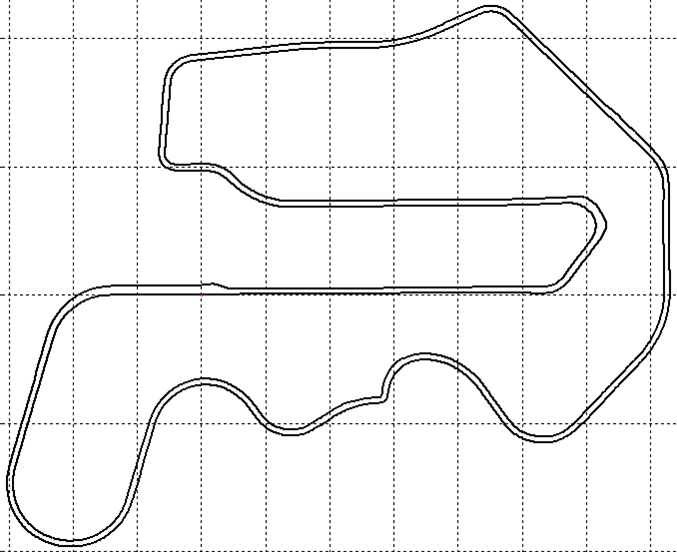
\includegraphics[width=2.7in]{figures/trackBoundaries.png}
\caption{Track boundaries of Thunderhill Raceway Park in Willows, CA. This is the racetrack frequently used for experimental data collection in the author's PhD laboratory.}
\label{fig:trackBoundaries}
\end{figure}
% % % % % % % end figure % % % % % % %

\subsection{Intuitive Solution From Racecar Drivers}
\label{sec:bro}

While optimal control methods have become increasingly popular in recent years due to advances in computing technology, professional racecar drivers have been qualitatively solving the
racing line problem for decades through years of practice and intuitive understanding of vehicle dynamics. In fact, former race car drivers have even written books qualitatively
explaining ideal driving trajectories (see, for example ``The Technique of Motor Racing" by former Formula One racer Piero Taruffi \cite{taruffi}).

% % % % % % % figure, blockdiagram % % % % % % %
\begin{figure}[h]
\centering
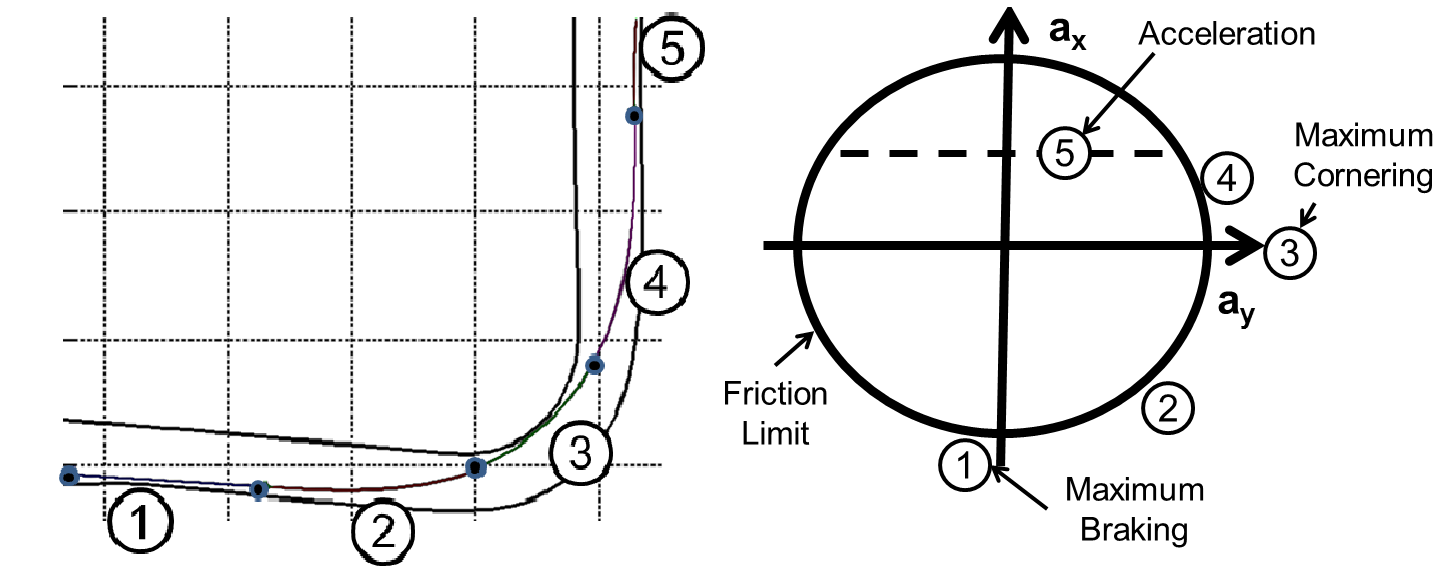
\includegraphics[width=3.25in]{figures/ggDiagram.png}
\caption{Typical racing line for 90 degree turn, with straight sections, constant radius section, and turn entry and exits. Each location of track corresponds to control strategy 
of driver on ``g-g" diagram.}
\label{fig:ggDiagram}
\end{figure}
% % % % % % % end figure % % % % % % %

The general approach taken by race car drivers is shown in Fig.~\ref{fig:ggDiagram}. Since available road-tire friction is limited, the driver will maximize the turning radius
by bringing the car to the outer edge of the track before turning inward to align the vehicle with the inner apex of the track. 
The turning maneuver completes with the car going back to the outer edge of the track boundaries. Fig.~\ref{fig:ggDiagram} also shows the ``g-g" diagram, or the limited vehicle longitudinal/lateral
acceleration capability resulting from tire friction limits. The driver will brake heavily in the straight section before the turn \textcircled{1}, before using a combination of braking and steering
at the turn entry \textcircled{2}, followed by pure cornering through the apex \textcircled{3}, followed by a combination of acceleration and steering at the turn exit \textcircled{4}. The driver finishes the turn by accelerating as fast
as the car's engine will allow \textcircled{5}.

  
 
%=======================================================================
\section{PRIOR WORK}
\label{sec:controller}

Given the practical interest by many racing teams in finding optimal lap times for different vehicle configurations, the optimal trajectory problem has been explored by several authors in
previously published literature. Hendrikx et al. in 1996 used optimal control theory and Pontryagin's minimum principle to come up with coupled differential equations to solve for the optimal trajectory
for a vehicle lane change maneuver \cite{hendrikx}. Casanova \cite{casanova} published a method  in 2000 for solving the minimum time racing problem using non-linear programming (NLP) in work
that was funded by the Benneton Formula One racing team. The NLP approach was further extended by Kelley \cite{kelly} in 2008, who extended Casanova's work to consider advanced effects such as transient 
vehicle dynamics and tire thermodynamics. 

More recently, the development of autonomous vehicle technology at the industry and academic level has led to research on optimal path planning algorithms that can be used for
driverless cars. Theodosis and Gerdes published a gradient-descent approach for determining optimal racing lines, with the racing line constrained to be composed of a fixed number of discrete
segments with linearly varying curvature \cite{theodosis}. The racing lines that result have feedforward steering and braking trajectories that are designed for an autonomous vehicle to follow, although
the path itself must be optimized off-line. Model predictive control (MPC) also offers the hope of real-time optimal path planning. Relevant work with racing lines generated by MPC include that of Gerdts in 2009 \cite{gerdts}, Prokop in 2010 \cite{prokop} and Timings and Cole in 2013 \cite{timings}.
Simulation results from these works have been encouraging, although the required computation time of these algorithms is roughly 1 second per time step using IBM's CPLEX solver, which is still a bit slow for real-time 
implementation on a race vehicle.


\section{PROJECT GOAL}

The goal of this project is to formulate the optimal racing line problem as a convex optimization problem that can be solved quickly in real time for the experimental Audi TTS testbed
shown in Fig.~\ref{fig:shelleyPic}. While this will require significant simplifications to the vehicle dynamics and the resulting control inputs, the hope is that the 
resulting racing line follows the general trends for minimum time racing shown in Section \ref{sec:bro}. With a known racing line, 
the problem of generating accurate feedforward control inputs can be solved quickly in real time,
 as shown by Kritiyakirana and Gerdes in 2012 \cite{mickgeneral}.

% % % % % % % figure, blockdiagram % % % % % % %
\begin{figure}[h]
\centering
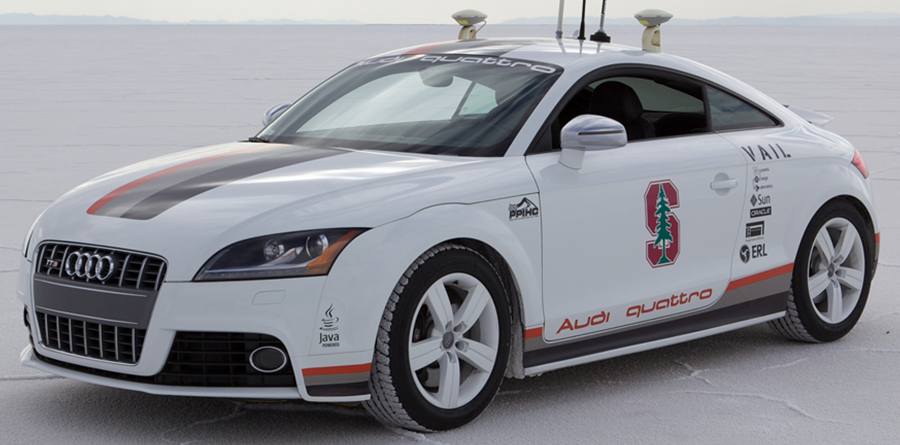
\includegraphics[width=3in]{figures/shelleyPic.png}
\caption{Audi TTS experimental testbed, equipped with differential GPS, drive and throttle by wire, and active brake booster.}
\label{fig:shelleyPic}
\end{figure}


\section{SIMULATION SETUP}
\subsection{Road Boundaries}
While the ultimate goal is to generate a racing line for the entire 16 turn course of Thunderhill shown in Fig.~\ref{fig:trackBoundaries},
for this final project, the preliminary goal is to find the optimal racing line for an arbitrarily chosen hairpin turn, parameterized by
path curvature as a function of distance along the path (Fig.~\ref{fig:roadPic}a). 
When plotted on East/North coordinate axes with a track width of 10 m, the resulting turn is shown in Fig.~\ref{fig:roadPic}b. 

\begin{figure}[h]
\centering
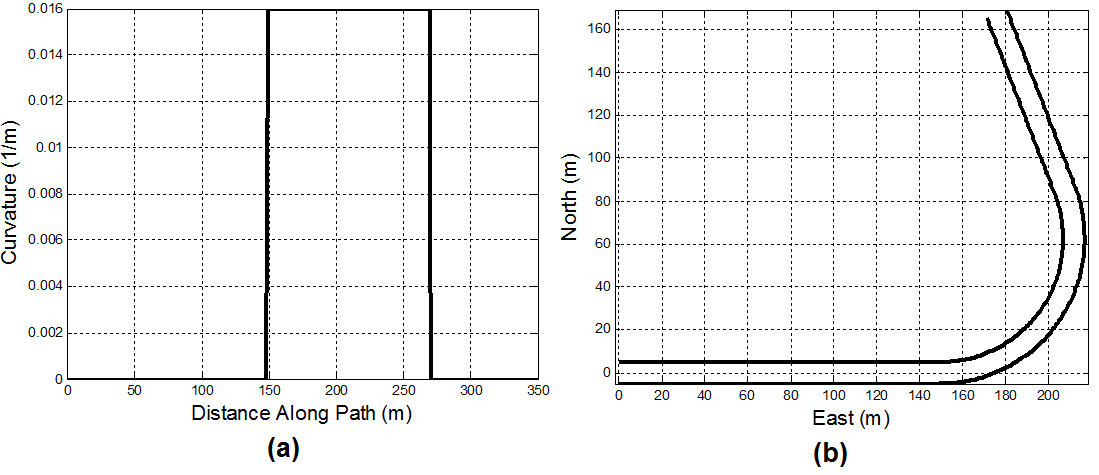
\includegraphics[width=3.5in]{figures/roadPic.png}
\caption{(a) Curvature profile of hairpin turn to be optimized. (b) Lane boundaries plotted on E-N coordinates.}
\label{fig:roadPic}
\end{figure}

\subsection{Linearized Vehicle Dynamics}

A commonly used vehicle dynamics model for path planning and general vehicle control is the two-wheel fixed-track model, shown
below in Fig.~\ref{fig:bikeModel}. 

\begin{figure}[h]
\centering
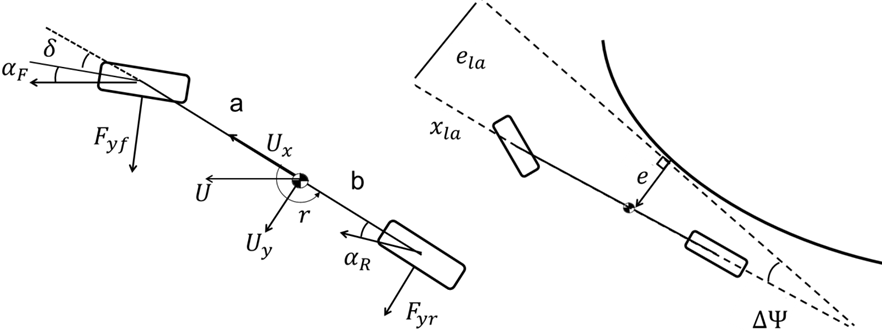
\includegraphics[width=3in]{figures/bikeModel.png}
\caption{(Left) Schematic of the two-wheeled vehicle model. (Right) Diagram showing path offset states $e$ and $\Delta\Psi$.}
\label{fig:bikeModel}
\end{figure}

The model has five states, with dynamics given as follows:

\begin{subequations}
\label{eqn:stateequations}
\begin{align}
        \dot{U}_\mathrm{y} & = \frac{F_\mathrm{yf} + F_\mathrm{yr}}{m}-rU_\mathrm{x} \\
        \dot{U}_\mathrm{x} & = \frac{F_\mathrm{xf} + F_\mathrm{xr}}{m}+rU_\mathrm{y} \\
				\dot{r}	   & = \frac{aF_\mathrm{yf} - bF_\mathrm{yr}}{I_\mathrm{z}}  \\
				\dot{e}    & = U_\mathrm{y} + U_\mathrm{x}\Delta\Psi \\
		\Delta\dot{\Psi}   & = r - U_\mathrm{x}\kappa
\end{align}
\end{subequations}

Where $U_\mathrm{y}$ and $U_\mathrm{x}$ are the vehicle lateral and longitudinal velocities, $r$ is the
vehicle yaw rate, $e$ is the vehicle offset from the path center line, and $\Delta\Psi$ is the vehicle heading error
from the path center line. The state derivatives depend on the lateral and longitudinal tire forces $F_\mathrm{y}$ and $F_\mathrm{x}$
at both the front and rear tires as well as the path curvature $\kappa$. The vehicle parameters $m$, $a$, $b$, and $I_z$ are given for
the Audi TTS test vehicle in Table 1. 

\begin{table}[h]
\small
\begin{center}
\caption{Vehicle Parameters}\label{tb:params}
\begin{tabular}{lccc}
Parameter & Symbol & Value & Units \\\hline
Vehicle mass & $m$ & 1500 & kg \\
Yaw moment of inertia & $I_z$ & 2250 & $\mathrm{kg \cdot m}^2$\\
Front axle to CG & $a$ & 1.04 & m\\
Rear axle to CG & $b$ & 1.42 & m \\\hline
\end{tabular}
\end{center}
\end{table}

Note that the vehicle state equations in (\ref{eqn:stateequations}) are nonlinear. Furthermore, generation of lateral tire
forces $F_\mathrm{yf}$ and $F_\mathrm{yr}$ are also nonlinearly dependent on the steering angle input $\delta$. These equations
of motion can therefore not be used as written in a convex optimization formulation. While Timings and Cole addressed this problem by linearizing
the state equations at every time step, we can simplify the vehicle dynamics by assuming that $U_\mathrm{x}$ is constant (i.e. $\dot{U}_\mathrm{x}$, $F_\mathrm{xf}$ and $F_\mathrm{xr}$ are all zero).
We will also assume a linear tire force model, where $F_\mathrm{yf}$ and $F_\mathrm{yr}$ are given by linear combinations of the steering input $\delta$ and the vehicle states.
These simplifications enable the vehicle dynamics to be modeled as a discrete time linear dynamical system.
 
\vspace{5 mm}
\subsection{Problem Formulation}

With the vehicle dynamics simplified, the optimization problem to solve is written as follows:

\begin{subequations}
\label{eq:OPT}
\begin{alignat}{3}
%% Objective Function
%\underset{F_\mathrm{yf,opt},S_\mathrm{sh,opt},S_\mathrm{env,opt}}{\text{minimize}} \quad & \left|F_{\mathrm{yf,driver}} -{F}_\mathrm{yf,opt}^{(0)}\right|
{\text{minimize}} \nonumber \\
& \sum_{k=1}^N \left|\left|\delta^{(k)} - \delta^{(k-1)} \right|\right|_1\label{eq:opt1}\\
%% Dynamic Constraints
\text{subject to}\nonumber\\
& \rlap{$ x^{(k+1)} = Ax^{(k)} + B\delta^{(k)}$} \label{eq:opt2}\\
& \rlap{$\left|{F_\mathrm{yf}}^{(k)}\right|\leq  \frac{\mu bg}{a+b}$}\label{eq:opt3}\\
& \rlap{$\left|{F_\mathrm{yr}}^{(k)}\right|\leq  \frac{\mu ag}{a+b}$}\label{eq:opt4}\\
& \rlap{$\left|\delta^{(k)} - \delta^{(k-1)} \right| \leq \Delta_\mathrm{max}$}\label{eq:opt5}\\
& \rlap{$e^{(k)} \leq w/2$} \label{eq:opt6}
\end{alignat}\label{eq:OPT}
\end{subequations}

An important observation from (\ref{eq:OPT}) is that the minimization criteria does not seek to minimize a time variable. Since we have
assumed a constant vehicle speed for the purpose of path planning, we can tune the speed $U_\mathrm{x}$ using a method such as bisection and determine
the maximum speed at which the optimization is feasible. The minimization criteria (\ref{eq:opt1}) is used instead to reduce the steering change between consecutive time steps.
This helps create the type of smooth driving paths that race car drivers take in practice. Moreover, use of the 1-norm is preferred since it tends to find steering inputs that are
piecewise linear, which are easy for experimental implementation. Using a constant speed also allows for a fixed number of time steps $N$ in the problem formulation.

The constraint in (\ref{eq:opt2}) ensures the solution follows the linearized, constant speed vehicle dynamics derived in the previous section, while constraints (\ref{eq:opt3})
and (\ref{eq:opt4}) enforce the tire friction limit for the front and rear tires, where $\mu$ is the estimated road friction. Constraint (\ref{eq:opt5}) enforces a slew rate limit on
the vehicle's steering input, where $\Delta_\mathrm{max}$ is the maximum steering change between time steps. Finally, (\ref{eq:opt6}) forces the vehicle to stay within the track boundaries
at all times, where $w$ is the track width and $e$ is the vehicle's lateral distance from the path centerline, which is one of the vehicle states in (\ref{eq:opt1}).

% % % % % % % end figure % % % % % % %

%=======================================================================
\section{SIMULATION RESULTS}
\label{sec:vvfb}

Fig.~\ref{fig:optPath} shows the results obtained by solving (\ref{eq:OPT}) using the CVX solver for convex optimization problems in MATLAB. The optimal
solution was obtained in 1.55 seconds of CPU time on an i7 laptop processor. The vehicle speed $U_\mathrm{x}$ for this solution was 24 m/s, with a lookahead 
horizon of $N =$ 300 time steps and a time step of .05 seconds
used for the discretization of the vehicle dynamics. The solution follows the general heuristics presented in Section \ref{sec:bro} in that
the computed trajectory starts and ends at the outer edges of the track and smoothly corners through the inner turn apex. 
 
\begin{figure}[h]
\centering
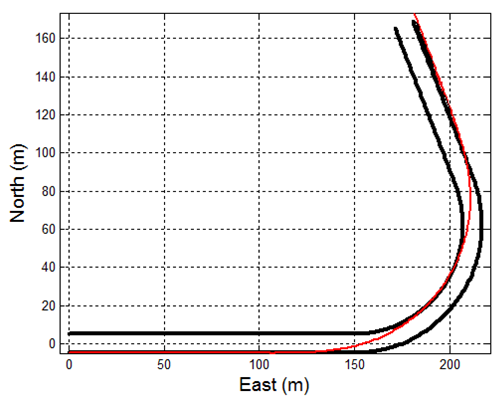
\includegraphics[width=3 in]{figures/optPath.png}
\caption{Optimal racing trajectory for hairpin turn.}
\label{fig:optPath}
\end{figure}

This result is further confirmed by plotting the path offset from the vehicle centerline as a function of time index $k$ in Fig.~\ref{fig:ePlot}. The result indicates
that the vehicle tends to stay at the outer edge of the track while on the straight track segments, while turning in at the apex.

\begin{figure}[h]
\centering
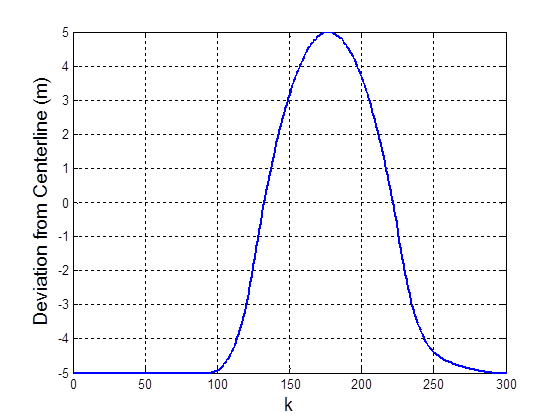
\includegraphics[width=3 in]{figures/ePlot.png}
\caption{Optimal path deviation for the hairpin turn as a function of time index $k$.}
\label{fig:ePlot}
\end{figure}

Fig.~\ref{fig:steerInput} shows the resulting steering control input in order to follow the optimal trajectory. One beneficial aspect
of the computed solution is that the resulting steering trajectory is piecewise linear, which allows the vehicle's curvature profile 
to be easily fit into the path planning structure
developed by Theodosis \cite{theodosis} and currently used on the Audi TTS testbed. 

\begin{figure}[h]
\centering
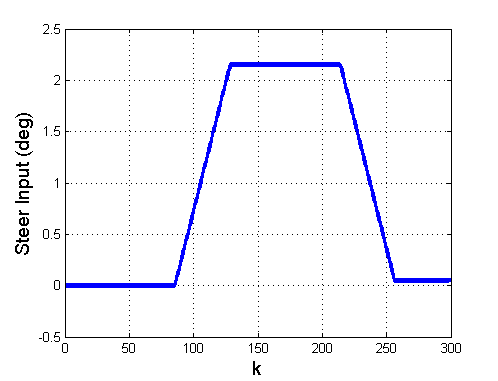
\includegraphics[width=3 in]{figures/steerInput.png}
\caption{Optimal steering input as a function of time index $k$.}
\label{fig:steerInput}
\end{figure}


%=======================================================================
\section{FUTURE WORK}

This work will likely be extended by the author into the Summer of 2014. Initial work to be done includes finding a simple way to compute
a reasonable estimate of the constant speed $U_\mathrm{x}$ for path planning purposes, instead of iterating to find the highest feasible
speed. Other work includes extending the solution from a simple turn to a race course with multiple turns, in which the path planner
will have to break the race course into turn-by-turn segments and ensure that continuity requirements are met between each turn. Additionally,
the planner may also have to lump several turns together if they occur in rapid succession. Finally, while CVX is an excellent solver
for initial proof of concept, commercially available packages such as CPLEX will need to be used for the vehicle to run a real time
path planner at a reasonable sampling rate. \\

%=======================================================================
\bibliography{Bibliography}  % bib file to produce the bibliography
\bibliographystyle{asmems4}

\end{document}